% ============================================================
% AIAA 2711 — Overfitting and Underfitting in Machine Learning
% Beamer Presentation — Spring 2025
% ============================================================
\documentclass[aspectratio=169, 10pt]{beamer}

% ---------- Theme ----------
\usetheme{Madrid}
\usecolortheme{default}
\setbeamertemplate{navigation symbols}{}
\setbeamertemplate{footline}[frame number]

% ---------- Packages ----------
\usepackage{amsmath, amssymb}
\usepackage{graphicx}
\usepackage{booktabs}
\usepackage{multicol}
\usepackage{xcolor}

% ---------- Figure path ----------
\graphicspath{{../report/figures/}}

% ---------- Custom commands ----------
\newcommand{\E}{\mathbb{E}}
\newcommand{\fhat}{\hat{f}}

% ---------- Title information ----------
\title{Overfitting and Underfitting in Machine Learning}
\subtitle{AIAA 2711 --- Spring 2025}
\author{Member A \and Member B \and Member C}
\date{}

% ============================================================
\begin{document}

% ---- Slide 1: Title ----
\begin{frame}
  \titlepage
  \note{Welcome everyone. Today we present our study on overfitting and underfitting in machine learning. (10s)}
\end{frame}

% ---- Slide 2: The Hook ----
\begin{frame}{The Hook: Which Model Do You Trust?}
  \begin{center}
    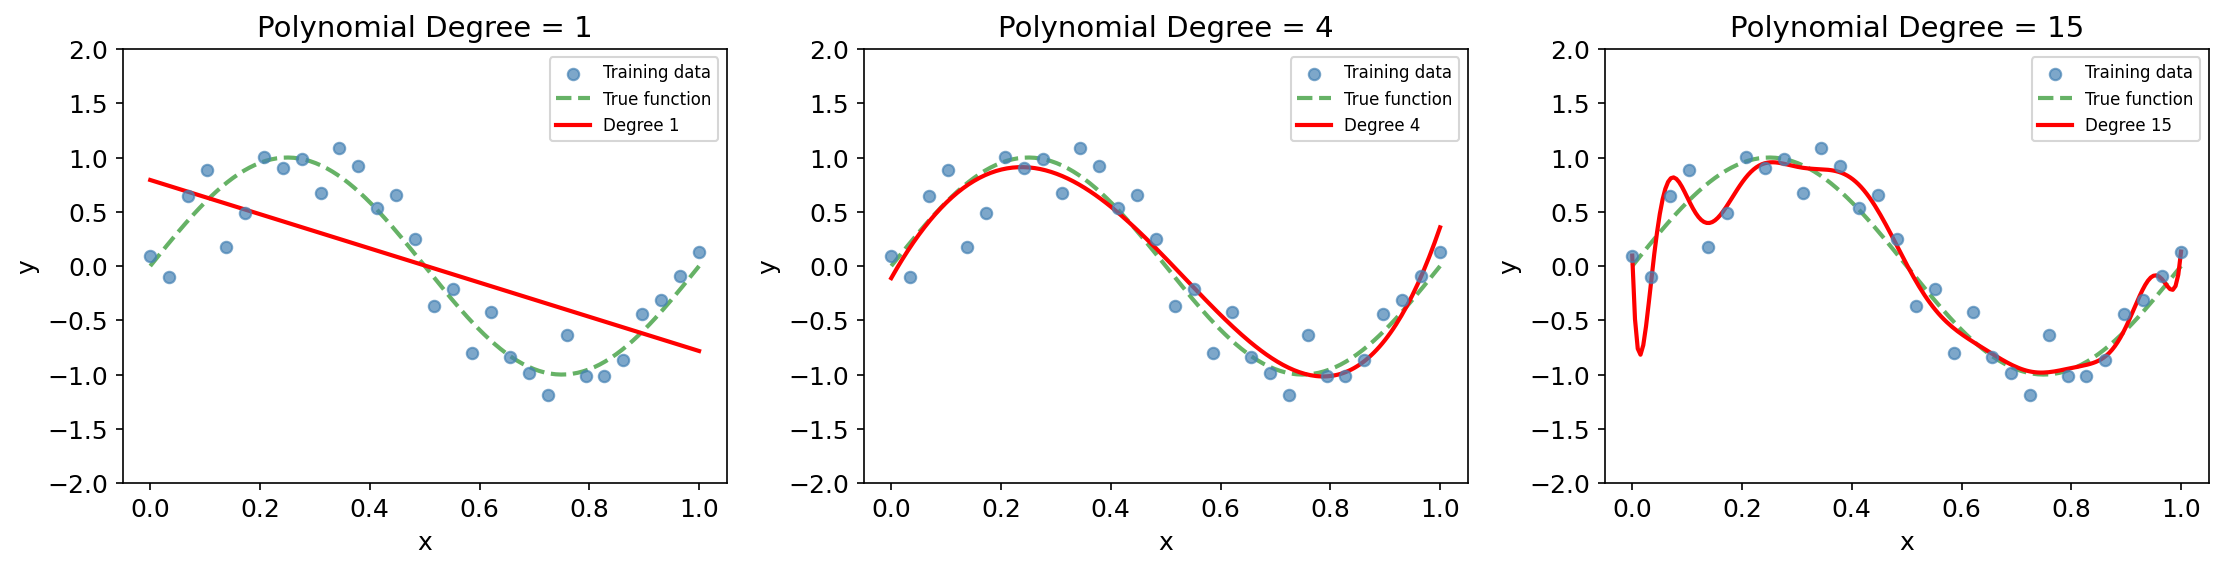
\includegraphics[width=0.85\textwidth]{polynomial_fits.png}
  \end{center}
  \vspace{0.3em}
  \begin{center}
    \textbf{Which polynomial would you trust to predict a new data point?}
  \end{center}
  \vfill
  {\footnotesize \textit{Vote by show of hands: degree 1, degree 4, or degree 15?}}
  \note{Speaker 1 asks audience to vote by show of hands for degree 1, 4, or 15. Most will pick degree 4 — we will explain why. (50s)}
\end{frame}

% ---- Slide 3: Formal Definitions ----
\begin{frame}{Formal Definitions}
  \textbf{Training Error:}
  \[
    E_{\text{train}} = \frac{1}{N}\sum_{i=1}^{N} \ell\bigl(y_i,\; \fhat(x_i)\bigr)
  \]

  \textbf{Test Error:}
  \[
    E_{\text{test}} = \E_{(x,y)\sim P}\bigl[\ell\bigl(y,\; \fhat(x)\bigr)\bigr]
  \]

  \vspace{0.5em}
  \begin{description}
    \item[Underfitting] $E_{\text{train}}$ high --- model too simple
    \item[Overfitting] $E_{\text{train}} \ll E_{\text{test}}$ --- generalization gap
  \end{description}

  \vfill
  \begin{block}{Key Message}
    The \textbf{generalization gap} is our diagnostic.
  \end{block}
  \note{Define training and test error formally. Underfitting = high training error; overfitting = large gap between train and test. (40s)}
\end{frame}

% ---- Slide 4: The Key Question ----
\begin{frame}{The Key Question: What Shapes the Error Curve?}
  \begin{columns}[T]
    \begin{column}{0.48\textwidth}
      \vspace{1em}
      \begin{itemize}
        \item Training error $\downarrow$ monotonically with complexity
        \item Test error is \textbf{U-shaped}
        \item Minimum near degree 3--5
      \end{itemize}
      \vfill
      \textbf{The answer:}\\
      Bias-Variance Decomposition\\
      {\small (uses expectation \& variance from Weeks 9--10)}
    \end{column}
    \begin{column}{0.48\textwidth}
      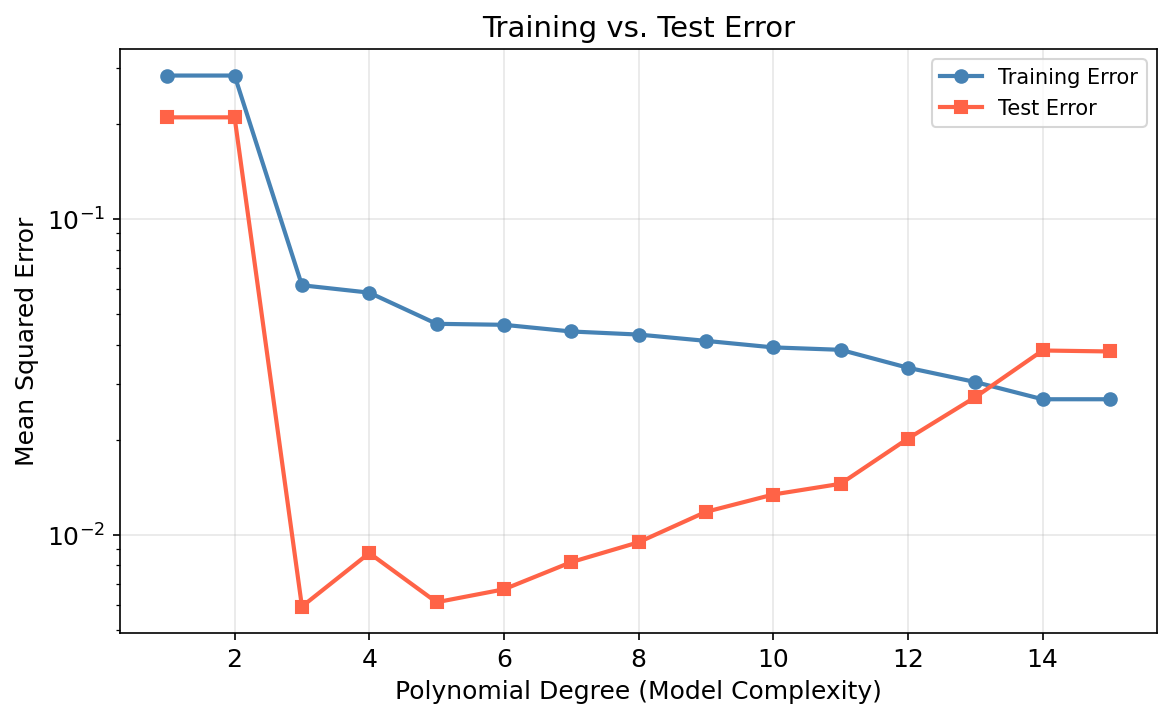
\includegraphics[width=\textwidth]{error_vs_complexity.png}
    \end{column}
  \end{columns}
  \note{Training error always decreases, but test error has a U-shape. The sweet spot is around degree 3--5. We explain this via bias-variance decomposition. (20s)}
\end{frame}

% ---- Slide 5: Bias-Variance Setup ----
\begin{frame}{Bias-Variance Setup}
  \textbf{Data model:}
  \[
    y = f(x) + \epsilon, \quad \epsilon \sim \mathcal{N}(0, \sigma^2)
  \]

  \vspace{0.5em}
  \begin{itemize}
    \item $f(x)$: true underlying function
    \item $\fhat(x)$: model trained on dataset $D$
  \end{itemize}

  \vspace{0.5em}
  \textbf{Goal:} decompose
  \[
    \E_D\bigl[(y - \fhat(x))^2\bigr]
  \]

  \vfill
  \begin{block}{Key Point}
    The expectation is over all possible training datasets $D$.
  \end{block}
  \note{Set up the bias-variance framework. The key insight is that we average over all possible training sets D. (40s)}
\end{frame}

% ---- Slide 6a: Bias-Variance Derivation — Steps (CORE) ----
\begin{frame}{Bias-Variance Derivation: Step-by-Step}
  \textbf{Step 1:} Expand $(y - \fhat)^2$ by substituting $y = f + \epsilon$:
  \pause
  \begin{align*}
    \E_D\bigl[(y - \fhat)^2\bigr]
    &= \E_D\bigl[(\underbrace{f - \fhat}_{\text{model error}} + \underbrace{\epsilon}_{\text{noise}})^2\bigr] \\
    &= \E_D\bigl[(f - \fhat)^2\bigr]
       + \E_D[\epsilon^2]
       + 2\,\E_D\bigl[\epsilon\,(f - \fhat)\bigr]
  \end{align*}

  \pause
  {\small \textbf{Cross-term:} $\epsilon$ is independent of $\fhat$ and $f$ is fixed,
  so $\E_D[\epsilon(f-\fhat)] = \E[\epsilon]\cdot\E_D[f-\fhat] = 0 \cdot (\ldots) = 0$.
  Also $\E_D[\epsilon^2]=\sigma^2$.}
  \[
    \boxed{\E_D\bigl[(y - \fhat)^2\bigr] = \E_D\bigl[(f - \fhat)^2\bigr] + \sigma^2}
  \]

  \pause
  \vspace{0.3em}
  \textbf{Step 2:} Now decompose $\E_D[(f-\fhat)^2]$. Let $\bar{f} \equiv \E_D[\fhat]$:
  \begin{align*}
    \E_D\bigl[(f-\fhat)^2\bigr]
    &= \E_D\bigl[(f - \bar{f} + \bar{f} - \fhat)^2\bigr] \\
    &= \underbrace{(f - \bar{f})^2}_{\text{constant}} + \E_D\bigl[(\fhat - \bar{f})^2\bigr]
       + 2(f-\bar{f})\,\underbrace{\E_D[\bar{f} - \fhat]}_{= \bar{f} - \bar{f} = 0}
  \end{align*}

  {\small \textbf{Cross-term:} $\E_D[\bar{f}-\fhat] = \bar{f} - \E_D[\fhat] = \bar{f} - \bar{f} = 0$.}

  \note{CORE SLIDE 6a. Walk through every line. Step 1: write out the full expansion with cross-term, explain independence kills it. Step 2: introduce shorthand f-bar, write out full expansion, explain the cross-term vanishes by definition of expectation. (50s)}
\end{frame}

% ---- Slide 6b: Bias-Variance Result + Monte Carlo Verification ----
\begin{frame}{Bias-Variance Decomposition: Result \& Verification}
  \begin{columns}[T]
    \begin{column}{0.55\textwidth}
      \textbf{Combining Steps 1 \& 2:}
      \[
        \boxed{
        \E_D[(y-\fhat)^2]
        = \underbrace{(f - \bar{f})^2}_{\text{Bias}^2}
        + \underbrace{\E_D[(\fhat - \bar{f})^2]}_{\text{Variance}}
        + \underbrace{\sigma^2}_{\text{Irreducible}}
        }
      \]
      \vspace{0.5em}
      \textbf{Interpretation:}
      \begin{itemize}
        \item \textbf{Bias$^2$}: average model's distance from truth\\
              {\small High bias $\rightarrow$ underfitting}
        \item \textbf{Variance}: prediction fluctuation across datasets\\
              {\small High variance $\rightarrow$ overfitting}
        \item $\boldsymbol{\sigma^2}$: noise floor --- no model can beat this
      \end{itemize}
      \vspace{0.3em}
      {\small Complexity $\uparrow$ $\Rightarrow$ Bias $\downarrow$, Variance $\uparrow$\\
      Complexity $\downarrow$ $\Rightarrow$ Bias $\uparrow$, Variance $\downarrow$}
    \end{column}
    \begin{column}{0.42\textwidth}
      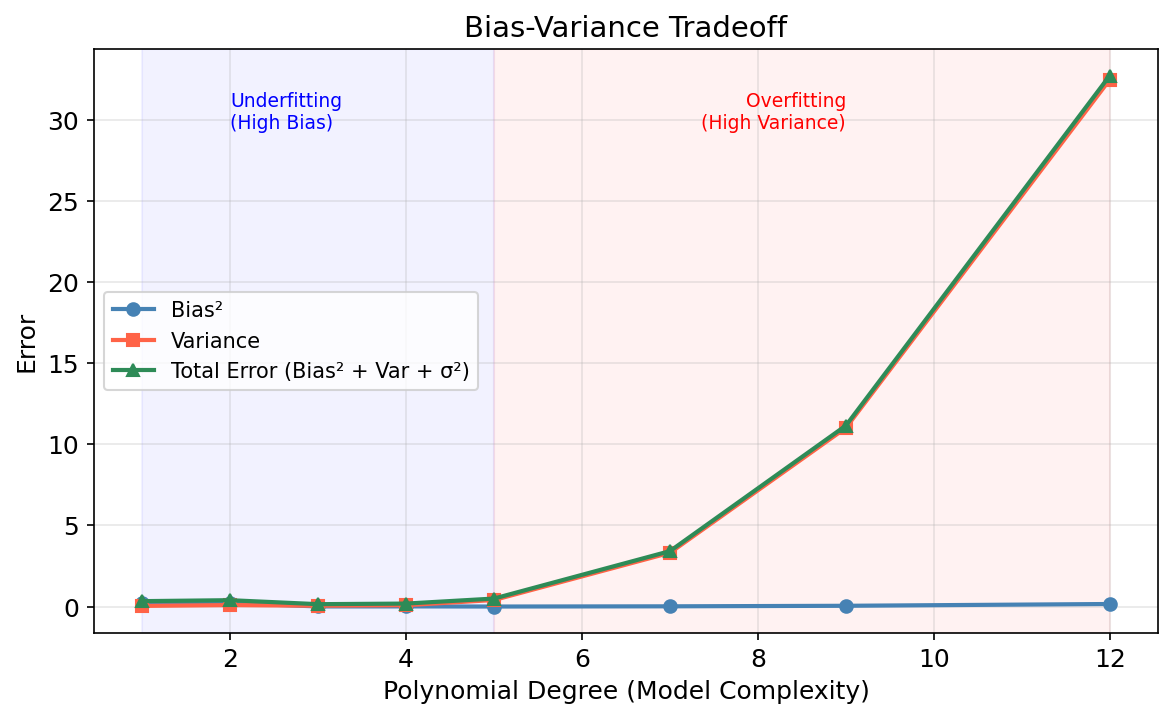
\includegraphics[width=\textwidth]{bias_variance_tradeoff.png}
      \vspace{0.2em}
      {\centering\small Monte Carlo verification\\(200 independent datasets)\par}
    \end{column}
  \end{columns}
  \note{CORE SLIDE 6b. Present the final boxed result. Interpret each term. Show the Monte Carlo figure: bias drops, variance rises, total error has a U-shape minimum near degree 3--4. (40s)}
\end{frame}

% ---- Slide 7: Regularization Motivation ----
\begin{frame}{Regularization: Constraining Complexity}
  High variance $\rightarrow$ overfitting.
  \textbf{Fix: constrain model complexity.}

  \vspace{1em}
  \begin{columns}[T]
    \begin{column}{0.45\textwidth}
      \textbf{OLS (no penalty):}
      \[
        \min_{\mathbf{w}} \|\mathbf{y} - \mathbf{Xw}\|_2^2
      \]
    \end{column}
    \begin{column}{0.45\textwidth}
      \textbf{Ridge ($\ell_2$ penalty):}
      \[
        \min_{\mathbf{w}} \|\mathbf{y} - \mathbf{Xw}\|_2^2 + \alpha\|\mathbf{w}\|_2^2
      \]
    \end{column}
  \end{columns}

  \vfill
  \begin{block}{Note}
    The $\ell_2$ norm is the Euclidean norm from Week 3.
  \end{block}
  \note{Transition from theory to practice. High variance means overfitting, and we fix it by adding a penalty term. Ridge adds an L2 penalty. (30s)}
\end{frame}

% ---- Slide 8: Ridge Closed-Form & Interpretations ----
\begin{frame}{Ridge: Closed-Form \& Interpretations}
  \textbf{Closed-form solution:}
  \[
    \mathbf{w}_{\text{ridge}} = (\mathbf{X}^\top\mathbf{X} + \alpha\mathbf{I})^{-1}\mathbf{X}^\top\mathbf{y}
  \]
  vs.\ OLS: $(\mathbf{X}^\top\mathbf{X})^{-1}\mathbf{X}^\top\mathbf{y}$

  \vspace{0.8em}
  \textbf{Two interpretations:}
  \begin{enumerate}
    \item \textbf{Eigenvalue (Week 5):}
      $\alpha\mathbf{I}$ shifts eigenvalues $\lambda_i \to \lambda_i + \alpha$, prevents instability when $\lambda_i \approx 0$.

    \item \textbf{Lagrangian (Week 9):}
      Equivalent to $\min \|\mathbf{y}-\mathbf{Xw}\|^2$ s.t.\ $\|\mathbf{w}\|^2 \leq t$;
      $\alpha$ is the Lagrange multiplier.
  \end{enumerate}

  \vfill
  \begin{block}{Key Insight}
    Adding $\alpha\mathbf{I}$ trades a small bias increase for a large variance decrease.
  \end{block}
  \note{Ridge has a clean closed form. The two interpretations connect to eigenvalues (Week 5) and Lagrangian duality (Week 9). The key trade-off: small bias increase buys large variance decrease. (80s)}
\end{frame}

% ---- Slide 9: Lasso & Geometric Comparison ----
\begin{frame}{Lasso \& Geometric Comparison}
  \textbf{Lasso ($\ell_1$ penalty):}
  \[
    \min_{\mathbf{w}} \|\mathbf{y} - \mathbf{Xw}\|_2^2 + \alpha\|\mathbf{w}\|_1
  \]

  \vspace{0.5em}
  \textbf{Geometric intuition:}
  \begin{itemize}
    \item $\ell_2$ ball (circle) $\rightarrow$ Ridge $\rightarrow$ smooth shrinkage
    \item $\ell_1$ ball (diamond) $\rightarrow$ corners on axes $\rightarrow$ \textbf{sparse solutions} (exact zeros)
  \end{itemize}

  \vspace{0.3em}
  \begin{center}
    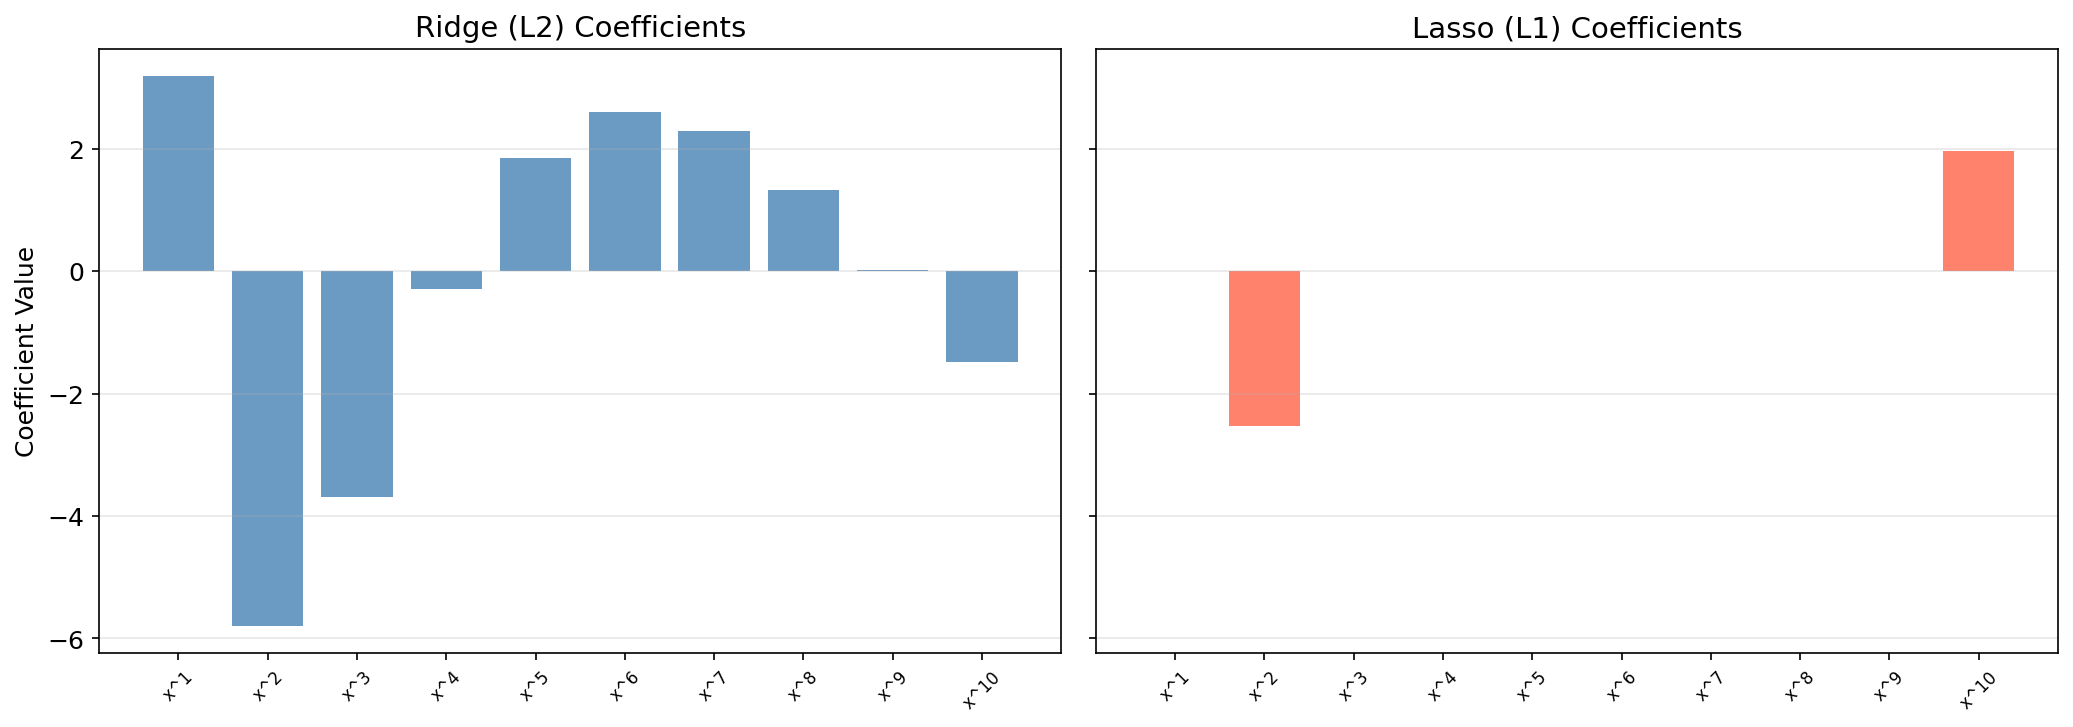
\includegraphics[width=0.55\textwidth]{ridge_vs_lasso_coefficients.png}
  \end{center}

  \vfill
  \textbf{Key insight:} Lasso = regularization + feature selection.
  \note{Lasso uses L1 penalty. Geometrically, the diamond shape of the L1 ball means solutions hit corners, producing exact zeros — automatic feature selection. (60s)}
\end{frame}

% ---- Slide 10: Cross-Validation ----
\begin{frame}{Cross-Validation: Choosing $\alpha$}
  \textbf{How to choose $\alpha$?} $K$-fold cross-validation.

  \vspace{0.8em}
  \begin{enumerate}
    \item Partition data into $K$ folds
    \item Train on $K{-}1$ folds, evaluate on fold $k$
    \item Average $K$ scores
    \item Select $\alpha$ minimizing CV error
  \end{enumerate}

  \vfill
  \begin{block}{Key Point}
    Unbiased test error estimate without a separate validation set.
  \end{block}
  \note{Cross-validation is the standard method for hyperparameter selection. K-fold gives an unbiased estimate of test error. (30s)}
\end{frame}

% ---- Slide 11: Experimental Verification ----
\begin{frame}{Experimental Verification}
  \textbf{Theory $\rightarrow$ Experiment mapping:}

  \vspace{0.5em}
  \begin{tabular}{@{}lll@{}}
    \toprule
    \textbf{Theory Prediction} & \textbf{Method} & \textbf{Result} \\
    \midrule
    U-shaped test error & Polynomial fits & Confirmed \\
    Bias$\downarrow$ Variance$\uparrow$ with complexity & Monte Carlo (200 datasets) & Confirmed \\
    Ridge shrinks coefficients & Ridge regression & Confirmed \\
    \bottomrule
  \end{tabular}

  \vspace{0.5em}
  \begin{center}
    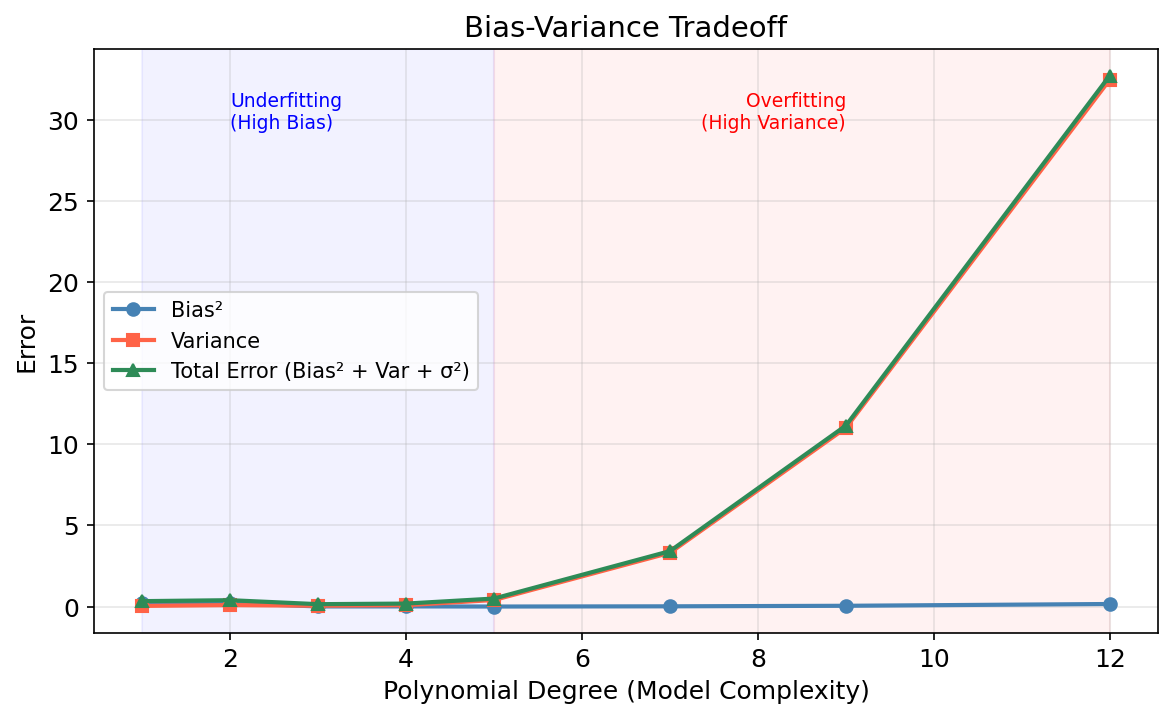
\includegraphics[width=0.55\textwidth]{bias_variance_tradeoff.png}
  \end{center}
  \note{All three theoretical predictions are confirmed experimentally. The Monte Carlo simulation with 200 datasets verifies the bias-variance decomposition. (50s)}
\end{frame}

% ---- Slide 12: Deep Learning Brief + Summary ----
\begin{frame}{Deep Learning \& Summary}
  \begin{columns}[T]
    \begin{column}{0.45\textwidth}
      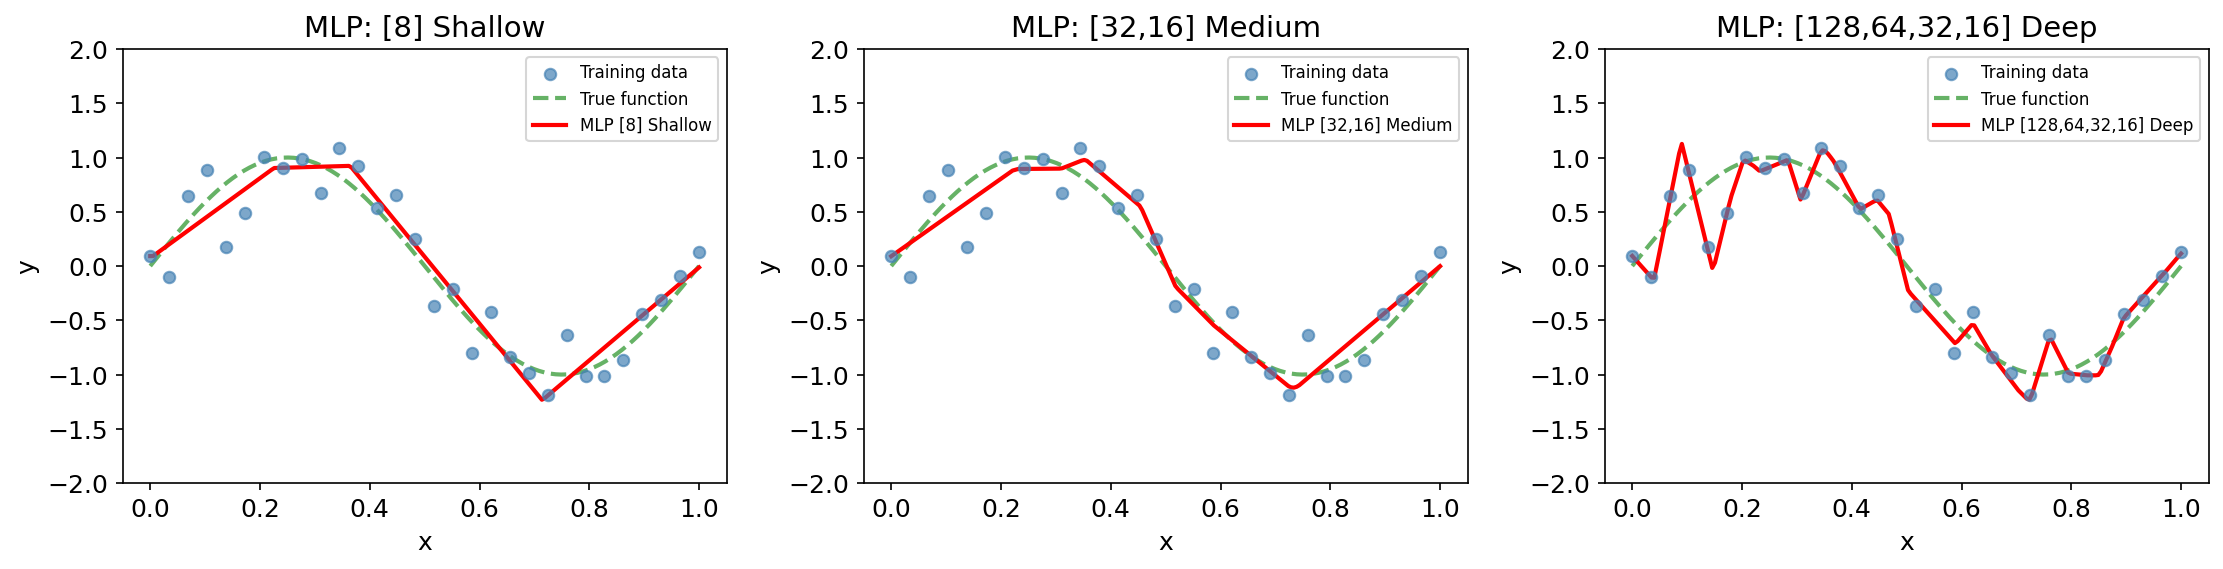
\includegraphics[width=\textwidth]{dl_synthetic_overfitting.png}
      \vspace{0.3em}
      {\small Same bias-variance principle applies to neural networks.}
    \end{column}
    \begin{column}{0.50\textwidth}
      \textbf{3 Key Takeaways:}
      \begin{enumerate}
        \item \textbf{Bias-Variance decomposition} explains the tradeoff mathematically
        \item \textbf{Regularization} (Ridge $\ell_2$ / Lasso $\ell_1$) controls complexity via norm penalties
        \item \textbf{Cross-validation} selects the optimal balance point
      \end{enumerate}
    \end{column}
  \end{columns}
  \note{The same principles extend to deep learning. Summarize the three main takeaways. (40s)}
\end{frame}

% ---- Slide 13: Interactive Closing + Q&A ----
\begin{frame}{Interactive Closing \& Q\&A}
  \textbf{Scenario:} A model achieves 99\% training accuracy but only 60\% test accuracy.

  \vspace{1em}
  \begin{itemize}
    \item \textbf{Q1:} Overfitting or underfitting?
    \item \textbf{Q2:} What is your fix?
  \end{itemize}

  \vspace{1em}
  \pause
  \textbf{Answer:}
  Generalization gap $= 39\%$ $\rightarrow$ \textbf{Overfitting}\\
  $\rightarrow$ Add regularization / reduce model complexity

  \vfill
  \begin{center}
    {\Large Thank You --- Questions?}
  \end{center}
  \note{Pose the scenario to the audience. Let them think, then reveal the answer. Generalization gap of 39 percent clearly indicates overfitting. (30s)}
\end{frame}

\end{document}
